\documentclass{fenicscourse}

\begin{document}

\fenicslecture{Lecture 19: FEniCS implementation}
              {Anders Logg}

\begin{frame}
  \frametitle{Key steps (linear PDEs)}

  \begin{enumerate}\setlength\itemsep{1em}
  \item
    Formulate linear variational problem: $a(u, v) = L(v)$
  \item
    Assemble linear system: $A = A(a)$ and $b = b(L)$
  \item
    Solve linear system: $U = A^{-1} b$
  \end{enumerate}

\end{frame}

\begin{frame}
  \frametitle{Key steps (nonlinear PDEs)}

  \begin{enumerate}\setlength\itemsep{1em}
  \item
    Formulate variational problem: $F(u) = 0$
  \item
    Differentiate variational problem: $F' = \partial F / \partial u$
  \item
    Solve nonlinear system:\\[1em]
    \begin{enumerate}\setlength\itemsep{1em}
    \item
      Assemble linear system: $A = A(F')$ and $b = b(F)$
    \item
      Solve linear system: $\delta U = -A^{-1} b$
    \item
      Update: $U \leftarrow U + \delta U$
    \end{enumerate}
  \end{enumerate}

\end{frame}

\begin{frame}
  \frametitle{Key steps for linear and nonlinear PDEs}

  \begin{enumerate}\setlength\itemsep{1em}
  \item
    Assemble linear system
  \item
    Solve linear system
  \end{enumerate}

\end{frame}

\begin{frame}
  \frametitle{Key data structures}

  \begin{itemize}\setlength\itemsep{1em}
  \item
    Meshes:
    \texttt{Mesh}
  \item
    Sparse matrices and vectors: \\
    \texttt{Matrix}, \texttt{Vector},
    \texttt{PETScMatrix}, \texttt{PETScVector}
  \item
    Functions:
    \texttt{Function}
  \item
    Dof maps:
    \texttt{DofMap}
  \end{itemize}

\end{frame}

\begin{frame}
  \frametitle{}
  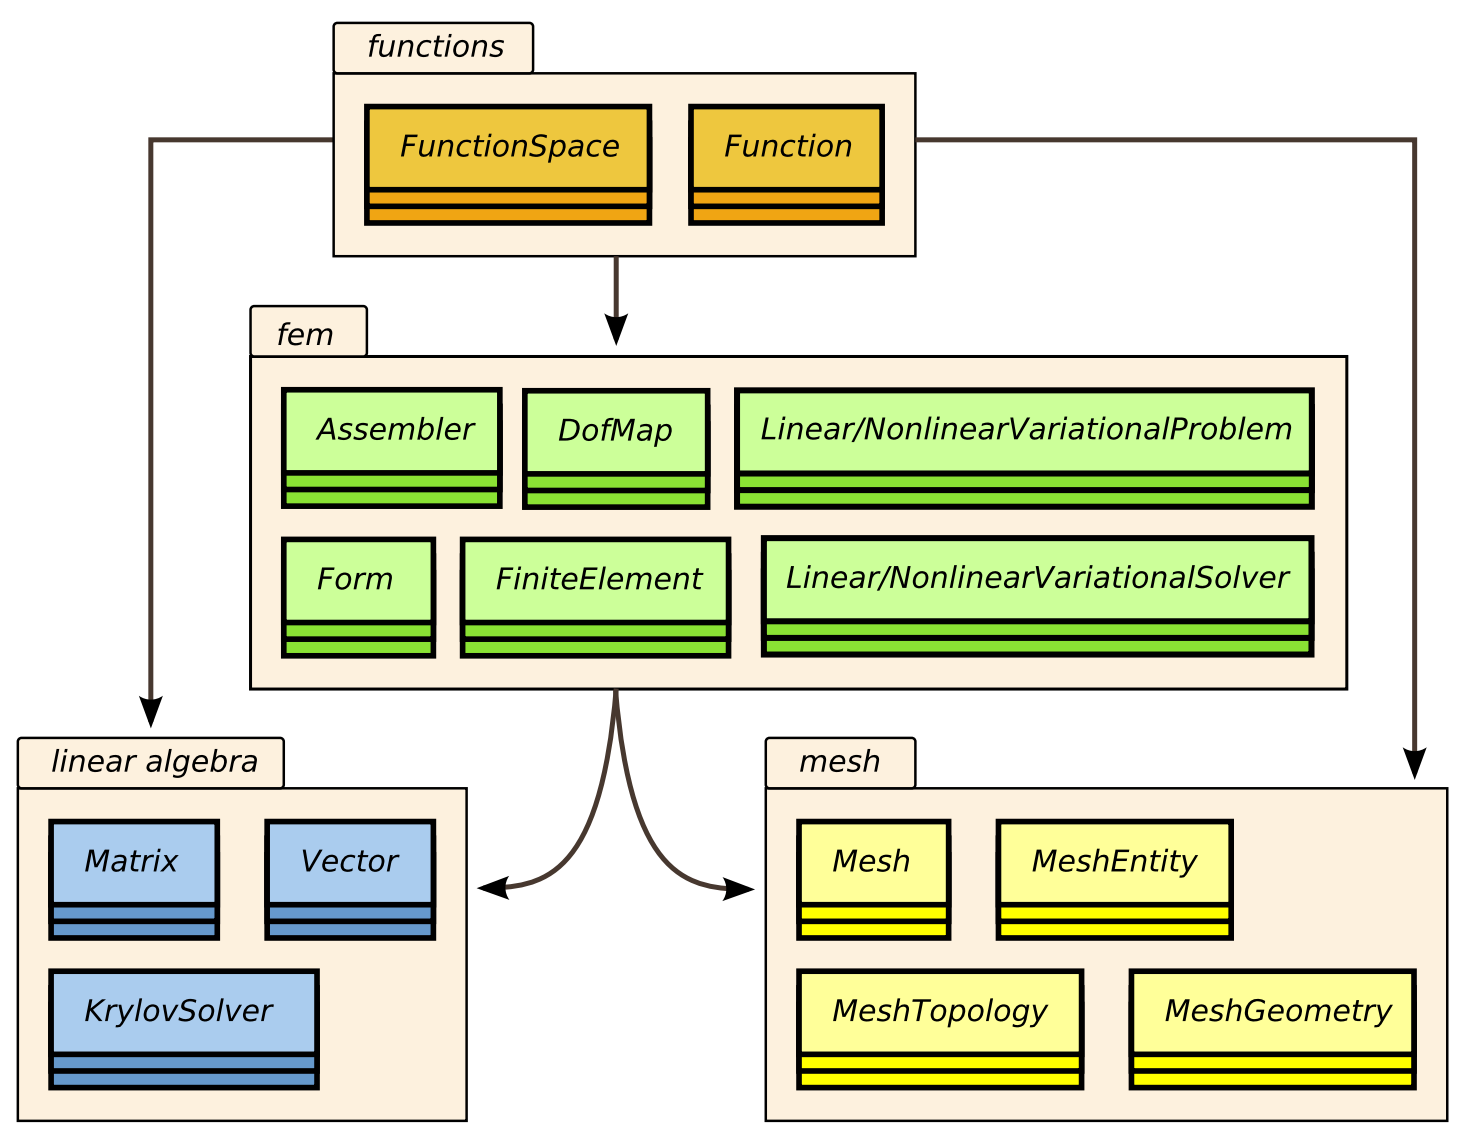
\includegraphics[width=\textwidth]{png/dolfin_classes.png}
\end{frame}

\begin{frame}
  \frametitle{Key algorithms}

  \begin{itemize}\setlength\itemsep{1em}
  \item
    Assembling linear systems: \texttt{Assembler} \\[1em]
    \begin{itemize}\setlength\itemsep{1em}
    \item
      Mapping degrees of freedom:
      \texttt{DofMapBuilder}
    \item
      Computing the element (stiffness) matrix:
      \texttt{ufc::tabulate\_tensor}
    \item
      Sparse matrix inseration:
      \texttt{Matrix.add()}
    \end{itemize}
  \item
    Solving linear systems: \\
    \texttt{LinearSolver}, \texttt{PETScKrylovSolver}
  \end{itemize}

\end{frame}

\begin{frame}[fragile]
  \frametitle{Mesh data structure}

  Separate mesh data into \emph{topology} (connectivity)
  and \emph{geometry} (coordinates).

  \bigskip

  From \texttt{dolfin/mesh/Mesh.h}:

\begin{c++}
class Mesh
{
public:
  ...
private:
  MeshTopology _topology;
  MeshGeometry _geometry;
};
\end{c++}

\end{frame}

\begin{frame}
  \frametitle{Mesh entities}
  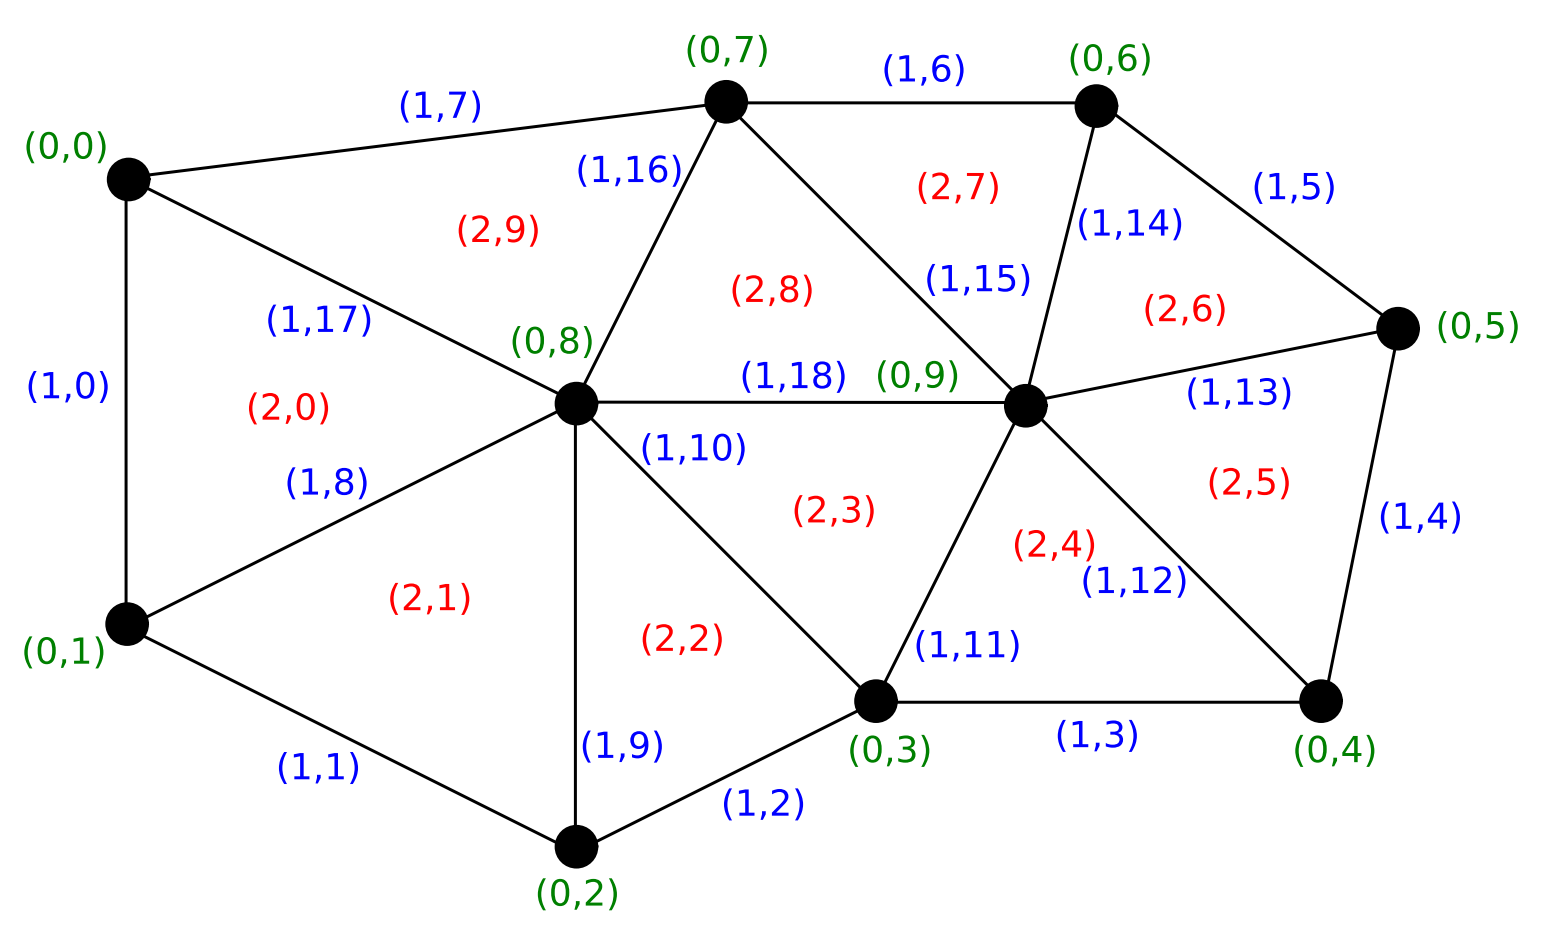
\includegraphics[width=\textwidth]{png/mesh_entities.png}
\end{frame}

\begin{frame}[fragile]
  \frametitle{Mesh topology}

  \bigskip

  From \texttt{dolfin/mesh/MeshTopology.h}:

  \bigskip

\begin{c++}
class MeshTopology
{
public:
  ...
private:
    std::vector<std::vector<MeshConnectivity> > connectivity;
};
\end{c++}

\end{frame}

\begin{frame}[fragile]
  \frametitle{Mesh connectivity}

  \bigskip

  From \texttt{dolfin/mesh/MeshConnectivity.h}:

  \bigskip

\begin{c++}
class MeshConnectivity
{
public:
  ...
private:
    std::vector<unsigned int> _connections;
    std::vector<unsigned int> _offsets;
};
\end{c++}

\end{frame}

\begin{frame}[fragile]
  \frametitle{Sparse matrix data structure}

  Sparse matrices in FEniCS are delegated to PETSc (or some
  other linear algebra backend).\\[1em]

  \bigskip

  Can otherwise be implemented using CRS (Compressed Row Storage):

\begin{c++}
class Matrix
{
public:
  ...
private:
   double* data;
   unsigned int* cols;
   unsigned int* offsets;
};
\end{c++}

\end{frame}

\begin{frame}
  \frametitle{Computing the sparse matrix $A$}

  \begin{itemize}
  \item
    $a = a(u, v)$ is a bilinear form (form of arity $2$)
  \item
    $A$ is a sparse matrix (tensor of rank $2$)
  \end{itemize}

  \bigskip

  \begin{equation*}
    A_{ij} = a(\phi_j, \phi_i)
  \end{equation*}

  \bigskip

  Note reverse order of indices!

\end{frame}

\begin{frame}
  \frametitle{Naive assembly algorithm}

  \begin{tabbing}
    $A = 0$ \\
    \\
    \textbf{for} $i=1,\ldots,N$ \\
    \\
    \tab \textbf{for} $j=1,\ldots,N$ \\
    \\
    \tab \tab $A_{ij} = a(\phi_j, \phi_i)$ \\
    \\
    \tab \textbf{end for} \\
    \\
    \textbf{end for}
  \end{tabbing}

\end{frame}

\begin{frame}
  \frametitle{The element matrix}

  The global matrix $A$ is defined by
  \begin{equation*}
    A_{ij} = a(\phi_j, \phi_i)
  \end{equation*}

  \bigskip

  The \emph{element matrix} $A_T$ is defined by
  \begin{equation*}
    A_{T,ij} = a_T(\phi_j^T, \phi_i^T)
  \end{equation*}

\end{frame}

\begin{frame}
  \frametitle{The local-to-global mapping}

  The global matrix $\iota_T$ is defined by
  \begin{equation*}
    I = \iota_T(i)
  \end{equation*}
  where $I$ is the \emph{global index} corresponding to
  the \emph{local index} i

  \begin{center}
    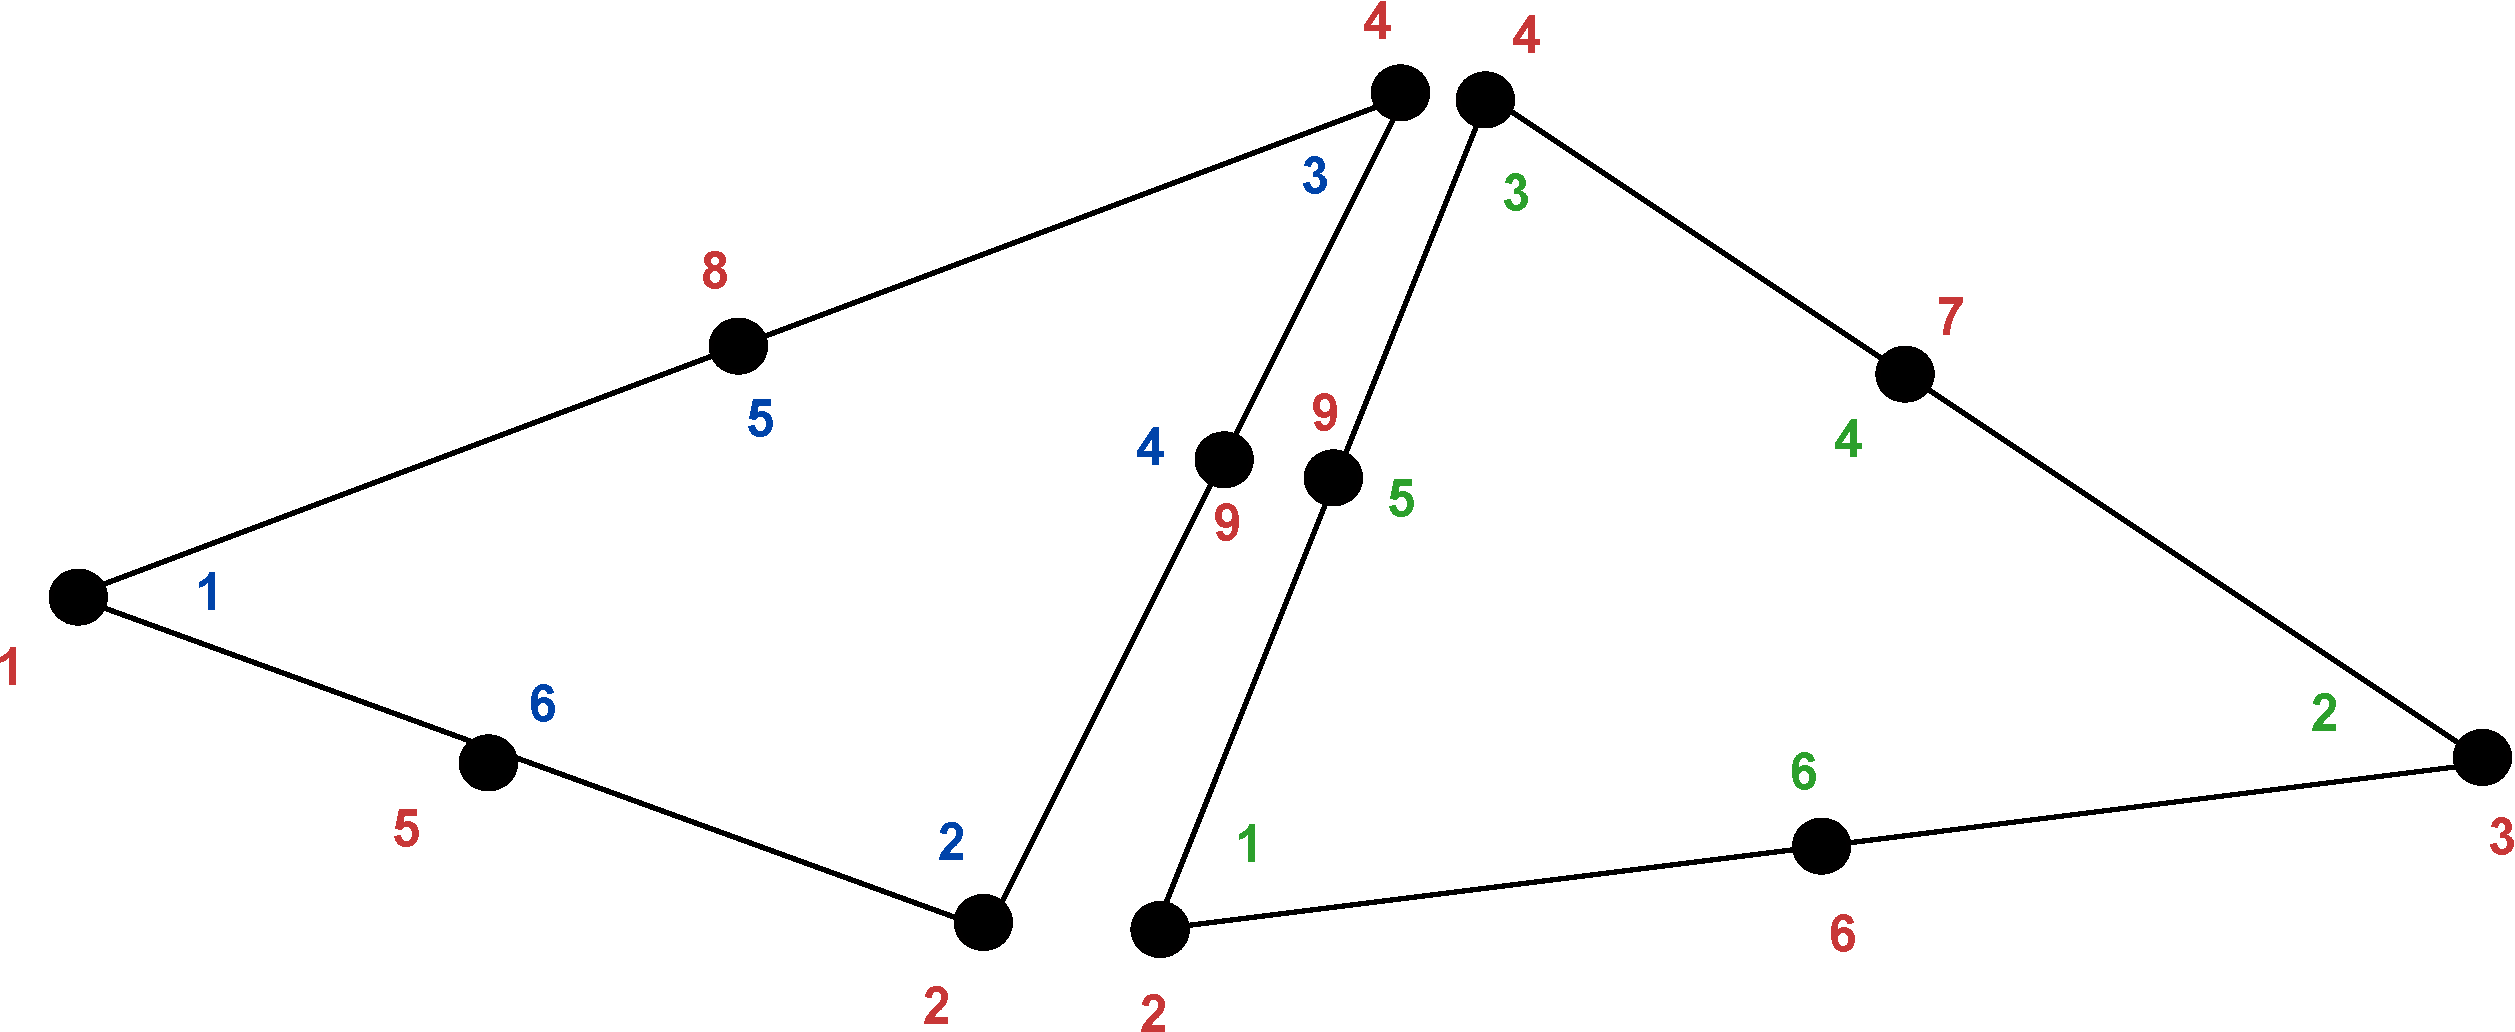
\includegraphics[width=10cm]{pdf/dofmap.pdf}
  \end{center}

\end{frame}

\begin{frame}
  \frametitle{The assembly algorithm}

  \begin{tabbing}
    $A = 0$ \\
    \\
    \textbf{for} $T \in \mathcal{T}$ \\
    \\
    \tab Compute the element matrix $A_T$ \\
    \\
    \tab Compute the local-to-global mapping $\iota_T$ \\
    \\
    \tab Add $A_T$ to $A$ according to $\iota_T$ \\
    \\
    \textbf{end for}
  \end{tabbing}

\end{frame}

\begin{frame}
  \frametitle{Adding the element matrix $A_T$}

  \begin{center}
    \def\svgwidth{\textwidth}
    \import{pdf/}{pdf/insertion.pdf_tex}
  \end{center}

\end{frame}


\begin{frame}
  \frametitle{Cell integrals and facet integrals}
  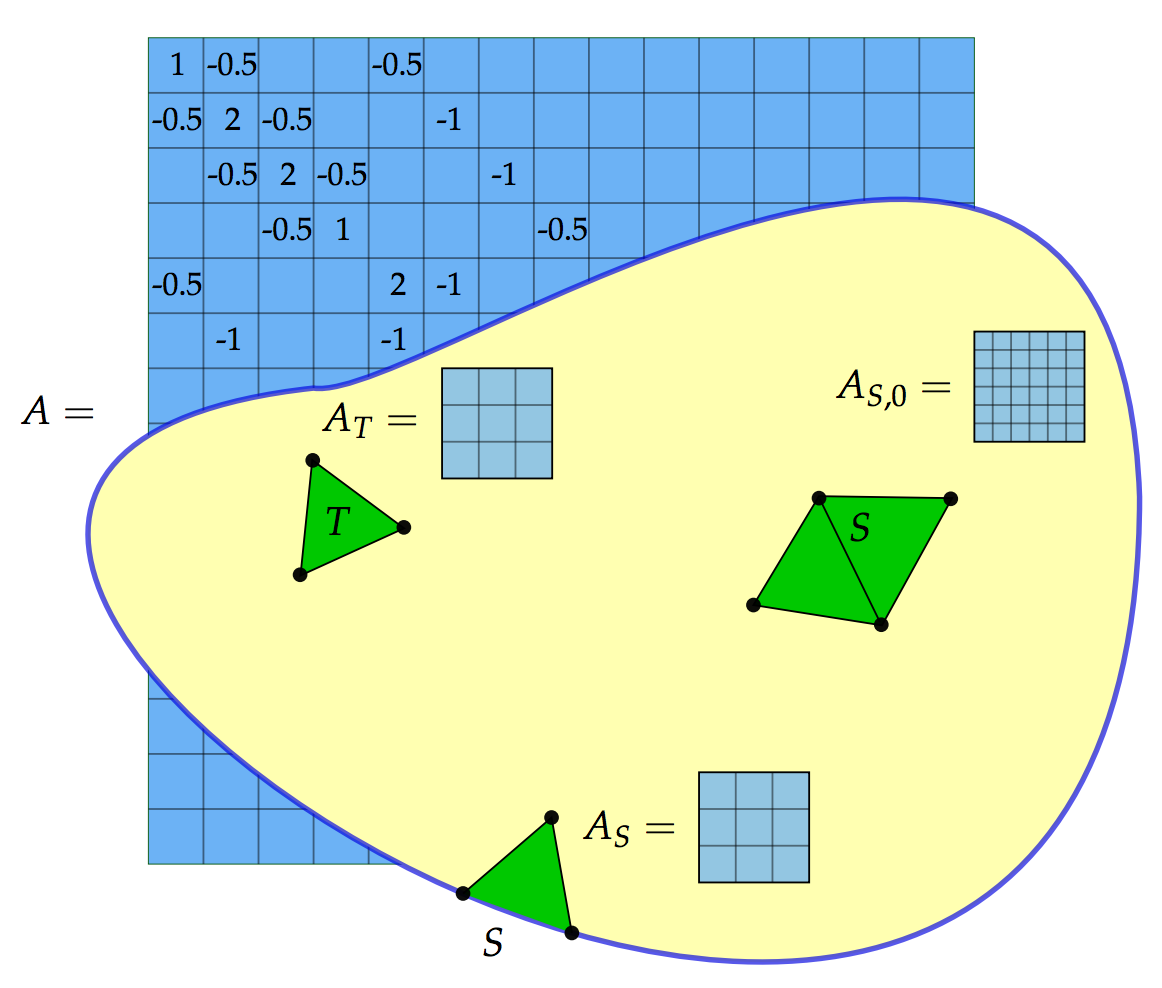
\includegraphics[width=0.9\textwidth]{png/assembly_integral_types.png}
\end{frame}

\begin{frame}
  \frametitle{FFC generates code for $A_T$}
  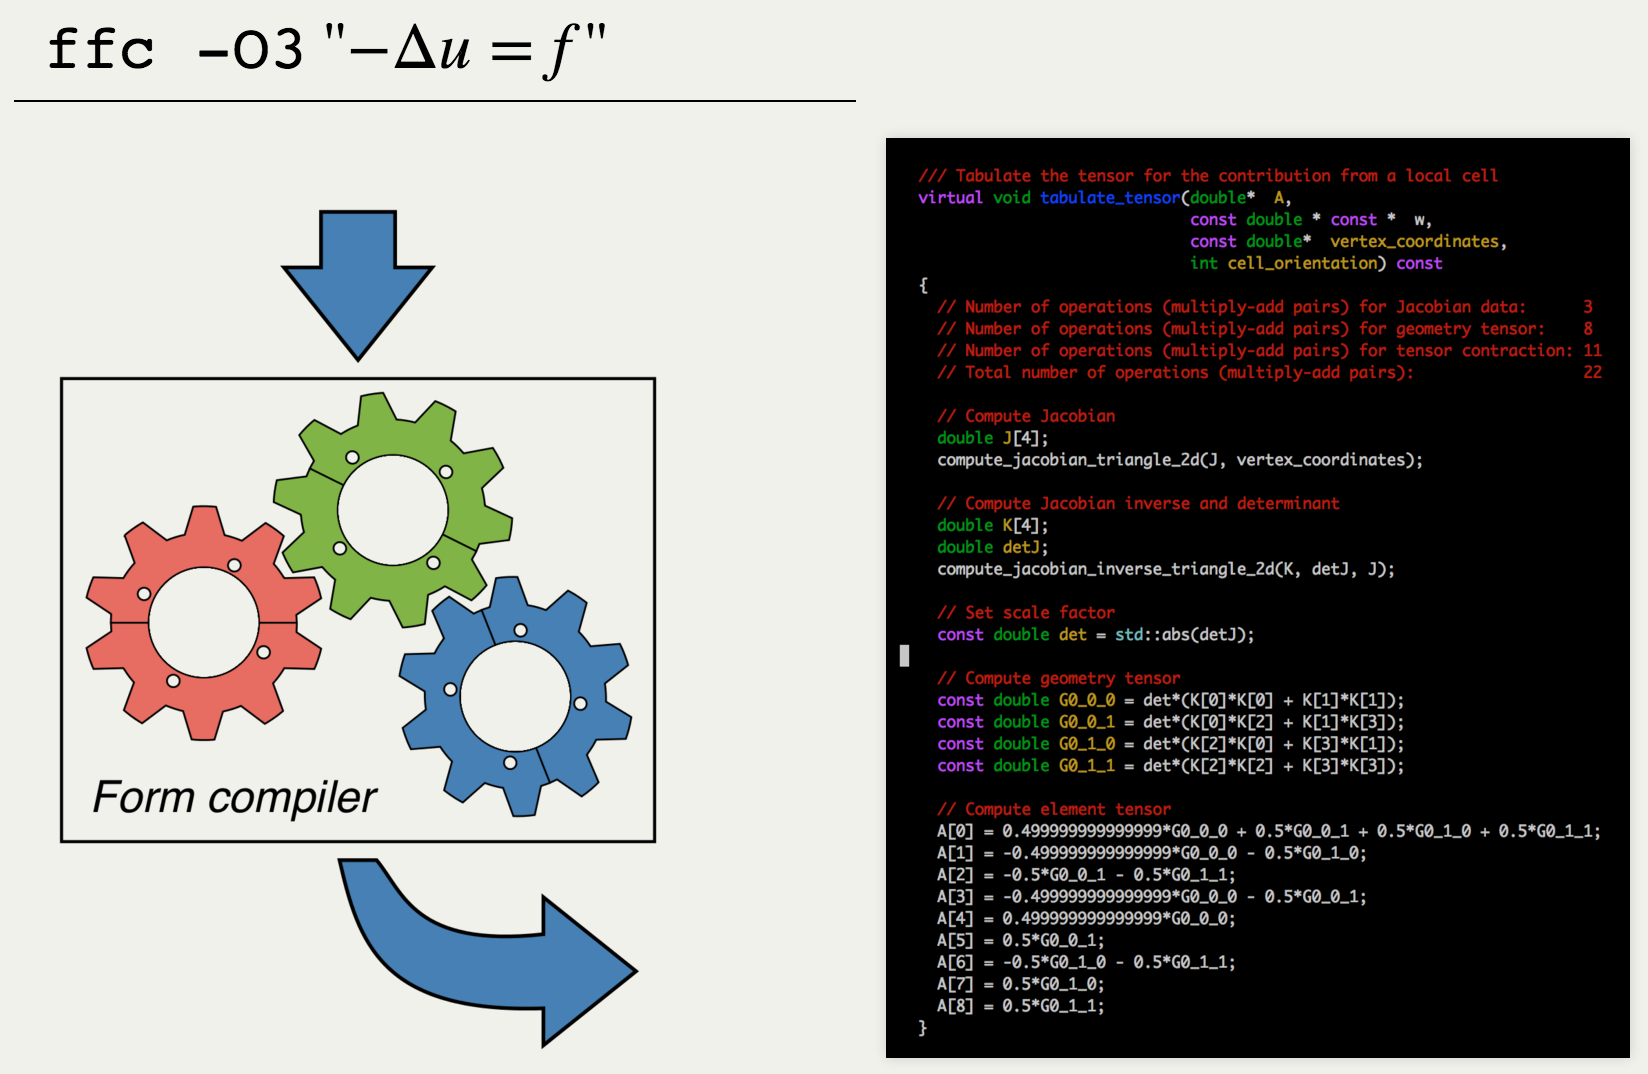
\includegraphics[width=\textwidth]{png/codegeneration_new.png}
\end{frame}

\begin{frame}
  \frametitle{Code generation chain}
  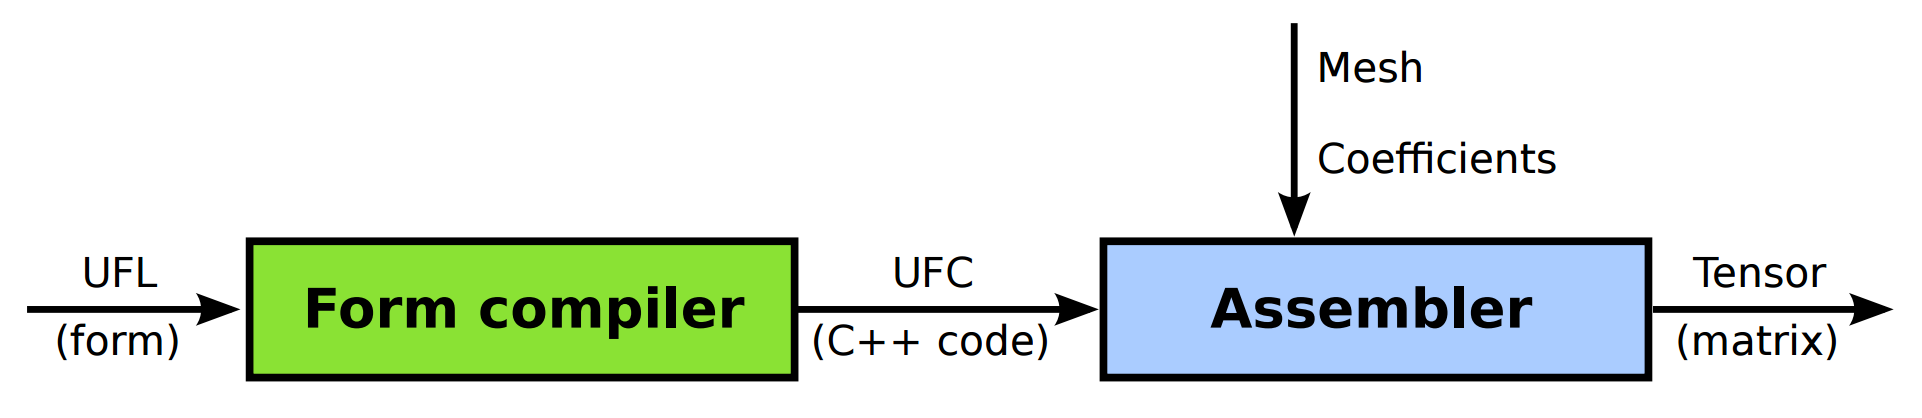
\includegraphics[width=\textwidth]{png/assembly_chain.png}
\end{frame}

\begin{frame}
  \frametitle{UFC data structures}
  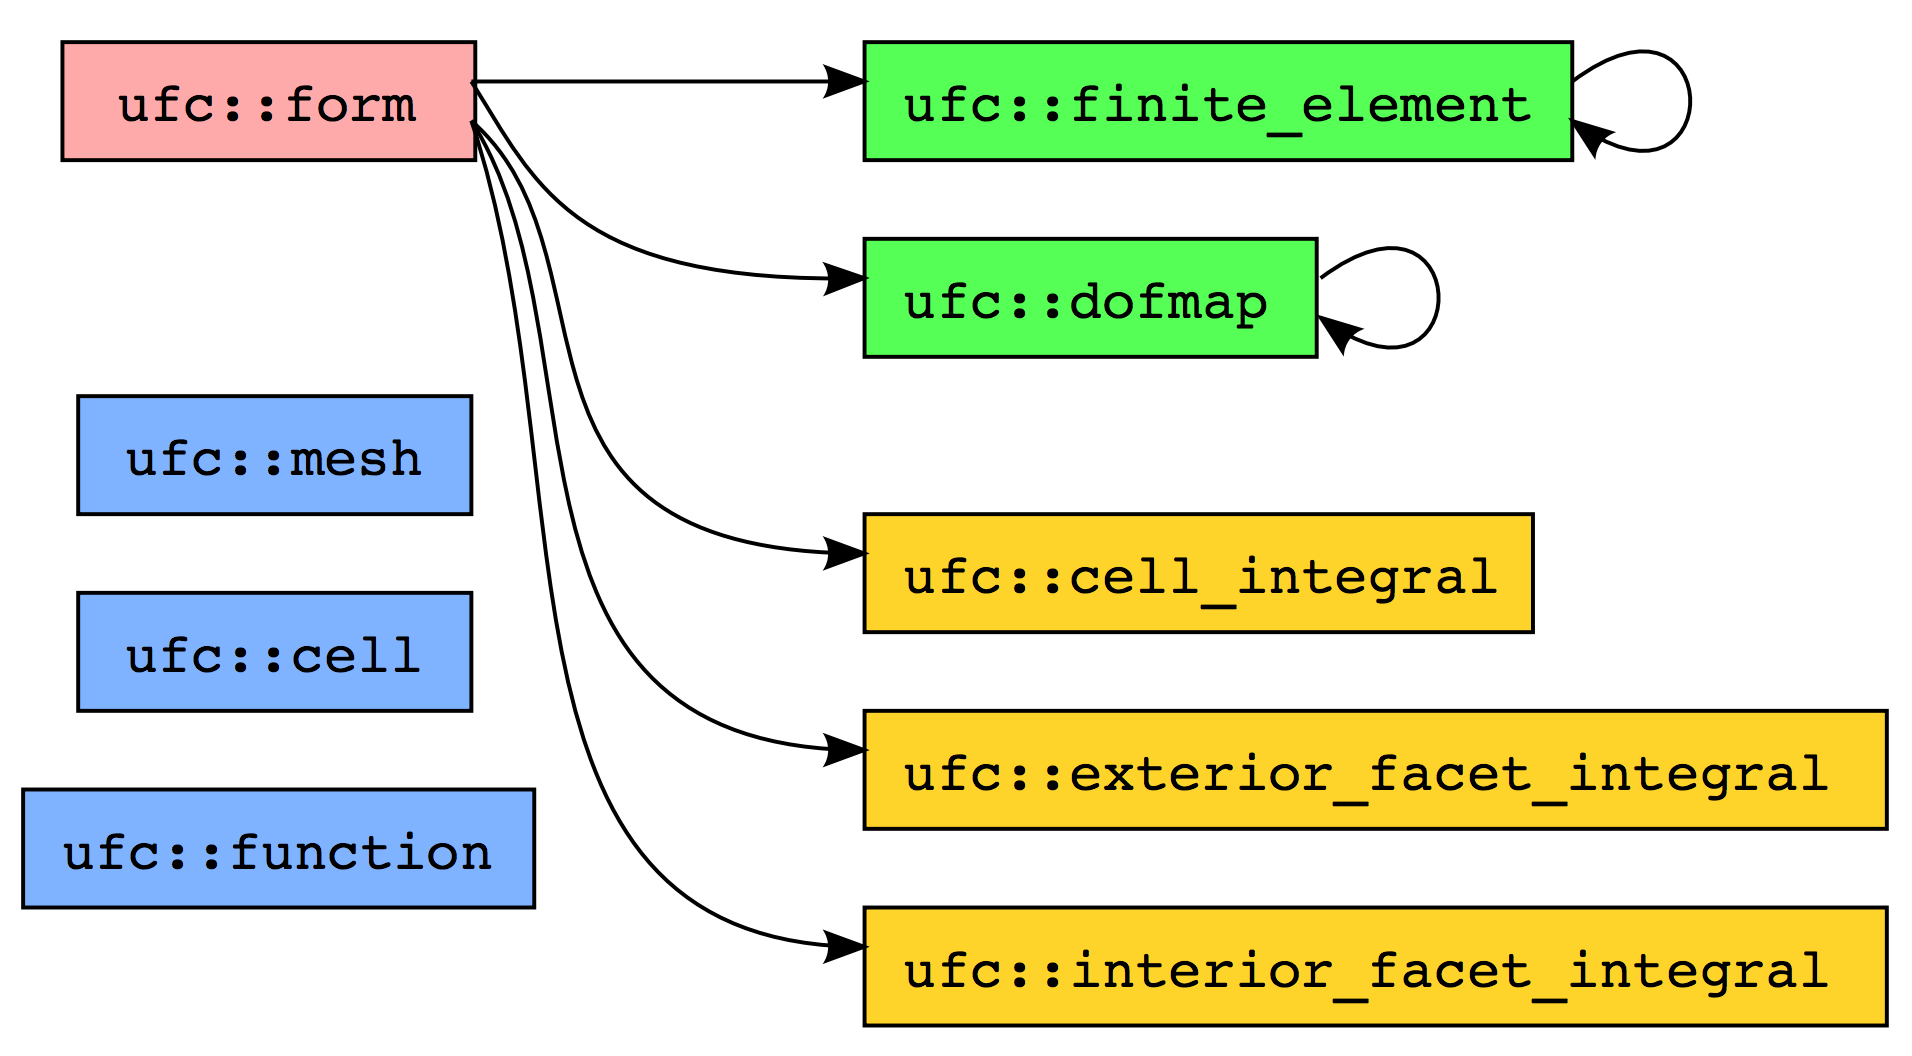
\includegraphics[width=\textwidth]{png/ufc_data_structures.png}
\end{frame}

\begin{frame}[fragile,shrink=10]
  \frametitle{The assembly implementation}

  \bigskip

  From \texttt{dolfin/fem/Assembler.cpp}:

  \bigskip

\begin{c++}
void assemble(GenericTensor& A, const Form& a)
{
  ...
  for (CellIterator cell(mesh); !cell.end(); ++cell)
  {
    for (std::size_t i = 0; i < form_rank; ++i)
      dofs[i] = dofmaps[i]->cell_dofs(cell->index());

    integral->tabulate_tensor(ufc.A.data(), ...);

    A.add_local(ufc.A.data(), dofs);
  }
}
\end{c++}

\end{frame}

\begin{frame}
  \frametitle{Iterative methods}

  Krylov subspace methods
  \begin{itemize}
  \item
    GMRES (Generalized Minimal RESidual method)
  \item
    CG (Conjugate Gradient method)
    \begin{itemize}
    \item
      Works if $A$ is symmetric and positive definite
    \end{itemize}
  \item
    BiCGSTAB, MINRES, TFQMR, \ldots
  \end{itemize}

  Multigrid methods
  \begin{itemize}
  \item
    GMG (Geometric MultiGrid)
  \item
    AMG (Algebraic MultiGrid)
  \end{itemize}

  Preconditioners
  \begin{itemize}
  \item
    ILU, ICC, SOR, AMG, Jacobi, block-Jacobi, additive Schwarz, \ldots
  \end{itemize}

\end{frame}


\begin{frame}[fragile]
  \frametitle{Solving linear systems}

  Iterative linear solvers in FEniCS are delegated to PETSc (or some
  other linear algebra backend).\\[1em]

  From \texttt{dolfin/la/PETScKrylovSolver.cpp}:

\begin{c++}
std::size_t solve(PETScVector& x,
                  const PETScVector& b)
{
  ...
  // Solve system
  ierr =  KSPSolve(_ksp, b.vec(), x.vec());
  if (ierr != 0) petsc_error(ierr, __FILE__, "KSPSolve");
  ...
}
\end{c++}

This function alone is 140 lines long. (!)
\end{frame}

\end{document}
